% 第 21 题【A】直角三角形图：按固定源 PDF 矢量路径换算（1 pt → 0.03515 cm）。
% 原点取 A 点（源页 (653.07, 180.07) pt），y 向上。
% A 左下、C 右下（AC 水平为斜边）、B 上方（直角顶点，∠ABC=90° 由题面保证）；
% D 为 B 到 AC 的垂足；E 为 BC 中点，连 DE。
% 注：源图为示意性（BA 与 BC 斜率积 ≈ −0.946，非严格垂直；图中未画直角记号），照源复刻。
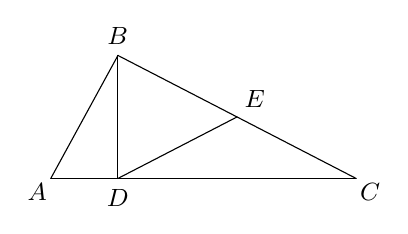
\begin{tikzpicture}[line cap=round,line join=round,font=\small,x=0.03515cm,y=0.03515cm]
\draw (0,0)--(24.26,44.43);      % A–B（直角边）
\draw (0,0)--(110.29,0);         % A–C（斜边，过 D）
\draw (24.26,44.43)--(24.26,0);  % B–D（斜边上的高）
\draw (24.26,0)--(67.28,22.21);  % D–E
\draw (24.26,44.43)--(110.29,0); % B–C（另一直角边，过 E）
% ===== 标注（照源字框中心，显式坐标）=====
\node[anchor=center,inner sep=0] at (-4.88,-4.76) {\(A\)};
\node[anchor=center,inner sep=0] at (24.21,51.39) {\(B\)};
\node[anchor=center,inner sep=0] at (115.36,-4.93) {\(C\)};
\node[anchor=center,inner sep=0] at (24.20,-6.98) {\(D\)};
\node[anchor=center,inner sep=0] at (73.66,28.53) {\(E\)};
\end{tikzpicture}
